\documentclass{article}
\usepackage{tikz}
\usepackage{verbatim}
\usepackage{amsmath}
\usetikzlibrary{positioning}
\begin{document}
\pagestyle{empty}
\centering
\begin{figure}[ht]
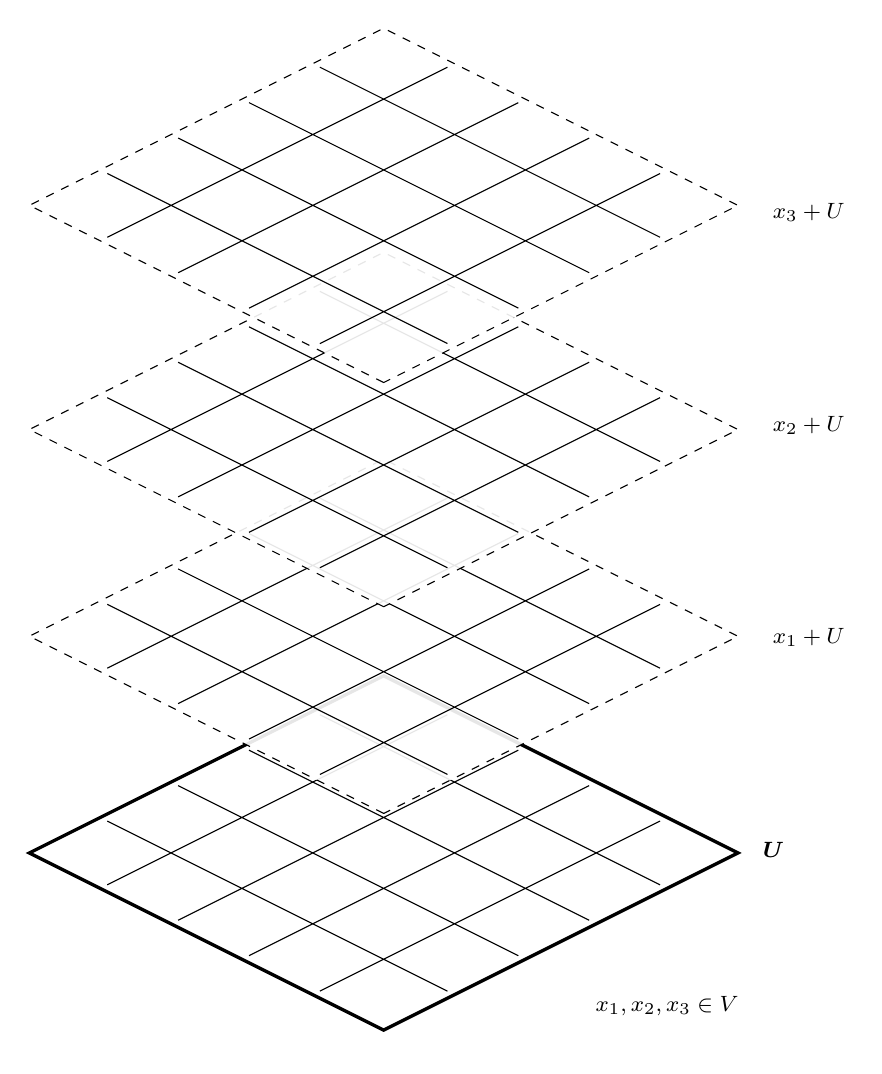
\begin{tikzpicture}[scale=.9,every node/.style={minimum size=1cm},on grid]

    \begin{scope}[ % bottom layer
      yshift=-170,every node/.append style={
      yslant=0.5,xslant=-1},yslant=0.5,xslant=-1
                 ]
      \fill[white,fill opacity=0.9] (0,0) rectangle (5,5);
      \draw[step=10mm, black] (0.1,0.1) grid (4.9,4.9);
      \draw[black,very thick] (0,0) rectangle (5,5);

      % \draw [fill=black](2.5,2.5) circle (.1) ;

    \end{scope}

    \begin{scope}[ % second from the bottom
       yshift=-83,every node/.append style={
       yslant=0.5,xslant=-1},yslant=0.5,xslant=-1
                 ]
      \fill[white,fill opacity=.9] (0,0) rectangle (5,5);
      \draw[step=10mm, black] (0.1,0.1) grid (4.9,4.9);
      \draw[black, dashed] (0,0) rectangle (5,5);
    \end{scope}
    	
    \begin{scope}[ % second from the top
    	yshift=0,every node/.append style={
    	yslant=0.5,xslant=-1},yslant=0.5,xslant=-1
    	           ]
      \fill[white,fill opacity=.9] (0,0) rectangle (5,5);
      \draw[step=10mm, black] (0.1,0.1) grid (4.9,4.9);
      \draw[black, dashed] (0,0) rectangle (5,5);
    \end{scope}
    	
    \begin{scope}[ % top layer
    	yshift=90,every node/.append style={
    	yslant=0.5,xslant=-1},yslant=0.5,xslant=-1
    	           ]
    	\fill[white,fill opacity=.9] (0,0) rectangle (5,5);
    	\draw[step=10mm, black] (0.1,0.1) grid (4.9,4.9);
    	\draw[black, dashed] (0,0) rectangle (5,5);
    \end{scope}  %end of drawing grids

    \fill[black,font=\footnotesize]
        (6,   5) node [above] {$x_3 + U$}
        (6,   2) node [above] {$x_2 + U$}
        (6,  -1) node [above] {$x_1 + U$}
        (5.5,-4) node [above] {$\boldsymbol{U}$}

        (4, -6.2)  node [above] {$x_1, x_2, x_3 \in V$};
\end{tikzpicture}
\end{figure}
\end{document}
